\chapter{OBSERVED QUANTITIES}
% !TEX root = hazy2.tex
\label{sec:ObservedQuantities}

\section{Overview}

This section describes how to convert the quantities actually used or
predicted by \Cloudy\ into commonly observed ones.

\section{Intensities of various continua}

\subsection{Incident radiation field}

The incident radiation field is the light striking the cloud.
The
main printout printout gives the intensity of the
incident radiation field with
the label ``Inci''.
The total continuum [units erg s$^{-1}$ or erg cm$^{-2}$~s$^{-1}$]
integrated over all energies is given with this label
and a wavelength of 0.
The incident
radiation field is also evaluated at two wavelengths,
4860 \AA\ and 1215 \AA ,
as $\lambda F_\lambda $ or $\nu F_\nu$,
[units erg s$^{-1}$ or erg~cm$^{-2}$~s$^{-1}$].

The \cdCommand{save continuum} command will produce a file that
contains the entire incident radiation field.

These entries will not be included if the \cdCommand{aperture} command
is in effect.

\subsection{The radiation field at specific wavelengths}

The intensity of the diffuse radiation field that is
emitted or reflected by the cloud is not normally included in the main output.
The \cdCommand{print continuum} command will include this radiation field
in the emission-line printout at a series of energies.  These have units
$\lambda F_\lambda $ or $\nu F_\nu$. See the discussion of the \cdCommand{print continuum}
and \cdCommand{set nFnu} commands in Part~1 for further details.
You can easily add more continuum points using the
\cdCommand{set nFnu add} command, also described in Part~1.

These entries will not be included if the \cdCommand{aperture} command
is in effect.

\subsection{The radiation field integrated over a range of wavelengths}
The emitted
radiation field integrated over a series of wavelength bands is included
in the main printout.
The file \cdFilename{continuum\_bands.ini} in the data
directory specifies a series of wavelength bands.
Table \ref{tab:continuum_bands} on page \pageref{tab:continuum_bands}
lists the default bands.
The label and wavelength
that are printed in the emission-line output are
given in the first two columns of that table.
The code
will integrate over these bands to find the total radiated
energy and report this in the main printout.
The \cdFilename{continuum\_bands.ini} file can be edited to change
the number of bands or their detailed properties.

This gives the \emph{total} emission that occurs over the band
and includes the incident radiation field and both line and continuum
diffuse emission.
Under many circumstances the radiation field within a band may be
dominated by the incident field.
The code can also report the emissivity in any of the emission
quantities given in the main printout.
For these continuum bands the emissivity will only be the
diffuse emission from the cloud and will not include the incident field.

These entries will not be included if the \cdCommand{aperture} command
is in effect.

\section{Emission-Line Equivalent Widths}

The equivalent width of an emission or absorption line is the number
of Angstroms of the continuum that is equivalent
to the energy in the line.
It is defined as
\begin{equation}
\label{eqn:EquivalentWidth}
W_\lambda =\int \frac{F_\lambda ^c-F_\lambda ^t}{F_\lambda ^c} d\lambda
\approx - \lambda \frac{F_{line}}{\lambda F_\lambda ^c}\quad
  [\mathrm{units\ of}~ \lambda]%(1)
\end{equation}
where the fluxes are in the incident continuum
($F_\lambda ^c$) and the line ($F_{line}$).
By this convention the equivalent width of an
emission line is negative.

The code's output can be used to predict a line's equivalent width.
The previous section describes several of the radiation fields
that are predicted.
The code prints the intensity or luminosity of all lines and continua and
the intensity of each relative to a normalization line.

The ratio of a line to continuum intensity or luminosity will be the
dimensionless ratio ${{{F_{line}}} \mathord{\left/
{\vphantom {{{F_{line}}} {\lambda \,F_\lambda ^c}}} \right.
 \kern-\nulldelimiterspace} {\lambda \,F_\lambda ^c}}$,
part of the last term in equation \ref{eqn:EquivalentWidth}.
The line equivalent width is
this ratio multiplied by the wavelength where the continuum is evaluated.
For instance, you could trick the code into printing
the relative intensities
of the lines as an equivalent width relative to the
incident radiation field at 1215 \AA\ by including the command
\begin{verbatim}
normalize to ``Inci'' 1215 scale factor = 1215
\end{verbatim}
This has two effects.
It gives the intensities relative to the
incident continuum at 1215 \AA\ and multiplies this by the continuum
wavelength in Angstroms, producing the rightmost ratio in equation 1.

A covering factor will complicate this slightly.
(Covering factors are
defined in the section \cdSectionTitle{Definitions} in Part I
of this document and in Section 5.9 of AGN3.)
In the luminosity case partial coverage of the source is
taken into account with the \cdCommand{covering factor} command
and the luminosities are correct for this coverage.
The ratio of line to continuum given in
equation \ref{eqn:EquivalentWidth} will represent what is observed.
In the intensity case the line
intensity is given per unit area of cloud no matter what covering factor
is specified.
In this second case the ratio in equation \ref{eqn:EquivalentWidth}
must be scaled by the covering factor.

\section{Emission-Line Asymmetries}

The inward fraction of the total emission of each line is always predicted
by the code.
It is not reported by default.
Many lines are significantly
inwardly beamed and this can lead to emission-line asymmetries if the
envelope is expanding.
The inward part of the lines will be printed if
the \cdCommand{print line inward} command is entered.
Note that the effects of this line beaming
are very geometry dependent.

\section{Surface Brightness}

\Cloudy\ will normally predict a line's intensity as $4\pi J$,
the intensity
radiated into $4\pi \sr$ by a unit area of cloud,
with units erg s$^{-1}$ cm$^{-2}$.
Observations of resolved sources often measure
the surface brightness, with
units erg s$^{-1}$ cm$^{-2}$ arcsec$^{-2}$ or
s$^{-1}$ cm$^{-2}$ sr$^{-1}$.
Be careful!  Some workers may report surface
brightness with units erg s$^{-1}$ cm$^{-2}$ arcsec$^{-2}$ sr$^{-1}$.
Remove the sr$^{-1}$ before
continuing by multiplying by $4\pi$.

To obtain the predicted surface brightness we must divide the intensity
$4\pi J$ by the number of square seconds of arc in $4\pi$~sr or the
number of sr in $4\pi$~sr.
One radian is $360/2\pi = 57.29578$ degrees,
so 1 sr is $(180/\pi)^2= 3282.806$ degree$^2$.
There are ${\left( {60 \times 60} \right)^2}$
square seconds in a square degree,
so there are $5.3464\times 10^{11}$ square arc
seconds in $4\pi$~sr.
The surface brightness (per square second of arc) is
the intensity $4\pi J$ multiplied by the inverse of this,
or $1.8704\times 10^{-12}$ arcsec$^{-2}$.
The surface brightness (per sr) is the intensity $4\pi J$ divided by $4 \pi$.

Note that this is only correct for a line that is emitted isotropically,
because the code predicts $4\pi J$ while an observer measures
$I$ along a particular direction.
(The code does predict the fraction of a line that is emitted
from the illuminated face of the cloud.)
This discussion is only formally
correct if $I = J$.

There is a
\cdCommand{print line surface brightness} command, 
described in 
Section~\ref{Hazy1-sec:CommandPrintLineSurfaceBrightness} 
\cdSectionTitle{\refname{Hazy1-sec:CommandPrintLineSurfaceBrightness}} 
of Hazy 1 which will change the intensity into
surface brightness units.
By default the final units will then be erg s$^{-1}$ cm$^{-2}$ sr$^{-1}$,
but the command has an \cdCommand{arcsec} keyword to specify the surface brightness
in erg s$^{-1}$ cm$^{-2}$ arcsec$^{-2}$.

\section{Flux to luminosity}

The luminosity is the intensity of a line multiplied by the total area
of the shell.
For full coverage this is $4\pi r^2$ where $r$ is the radius of the shell.
If the shell only partially covers the continuum source then this
should be multiplied by the covering factor.

\section{Flux at the Earth}

If the distance to the object is specified with the
\cdCommand{distance} command,
and the luminosity case is predicted then the flux observed at the Earth
will be predicted if the \cdCommand{print flux at Earth} command
also appears.

\section{Relative hydrogen line intensities}

Hydrogen line intensities can be predicted with great precision when
Case B applies.
\citet{FergusonFerland1997} describe \Cloudy's
original hydrogen atom and
\citet{FerlandFabianEtAl2009} describe its current implementation.
It gives good results for all reported lines.
The number of reported lines can be increased to go higher in
the \hi\ model atom
by using the \cdCommand{atom H-like levels} command.
This gives better results at
the expense of more compute time.

The accuracy of \Cloudy's \hi\ line emissivities is limited by the size
of the model hydrogen atom that can be computed on the fly.
The definitive
calculation for hydrogen recombination is that of \citet{Hummer1987}
and \citet{Storey1995}, who used a 1000 level atom with all $l$-levels
explicitly considered
(that works out to something like a million levels!).
The code interpolates on their tables and includes their Case A and Case
B predictions within the main printout.
The test cases \cdFilename{limit\_case*.in} in the test suite
compare the code's predictions with their Case~B values.

The \citet{Hummer1987} calculation is for Case B conditions, which
assume that many processes are unimportant (see AGN3).
Neglected processes include collisional excitation from the
ground or first excited states, induced processes where the incident
continuum causes the atom to fluoresce, and line transfer in all non-Lyman
lines.
Case~B is often an excellent assumption for galactic nebulae such
as planetary nebulae or H II regions.
Case~B is not valid for gas densities
greater than $10^6 \pcc$ or when X-rays are present.
When any of these
processes are important the
predictions of \Cloudy's model atom are more realistic than Case~B
predictions.

\section{Helium line intensities}

The code includes a model of the He$^0$ atom that is applied all along the
helium iso-electronic sequence.
The model can have an arbitrarily large
number of levels (\citealp{Bauman2005}; \citealp{Porter2005}; \citealp{PorterFerland2007}).
The predictions become more exact as the number of levels is
increased.

\section{Line Intensities in a dusty open geometry}

Two sets of line intensities are printed.
The first block of lines,
with the title ``Intrinsic~Intensities'',
includes all the physics of line
formation but does not include the effects of absorption and scattering
of the line from regions away from that were the line forms. This would
be the spectrum you would observe after correction for reddening or line
of sight extinction.

The second block of emission-line intensities, with the title
``Emergent~Intensities'',
includes the effects of absorption and scattering from regions
outside those where the lines form.
The distinction is important for a
dusty open geometry.
This geometry is appropriate for the Orion Nebula,
a blister H II region on the surface of Orion Molecular Cloud 1 (OMC1).
An idealized geometry is shown in Figure \ref{fig:DustyOpenGeometry}.
The code computes the fraction
of the line emission that is directed towards the illuminated and shielded
faces.  The outward line emission is emitted towards the PDR that may have
a large optical depth due to grains.  The albedo of the gas-grain mixture
is computed and the fraction reflected is passed back towards the illuminated
face.  The total intensities are roughly half what would be expected were
the cloud emitting from both sides.  Something like 10\% of the light
striking the molecular cloud will be reflected back to the observer, and
so slightly more than 50\% of isotropically emitted lines will emerge from
the illuminated face.  The code uses the albedo of the gas at the wavelength
of the line to predict this reflected portion and the full optical depths
computed on previous iterations.

\begin{figure}
\centering
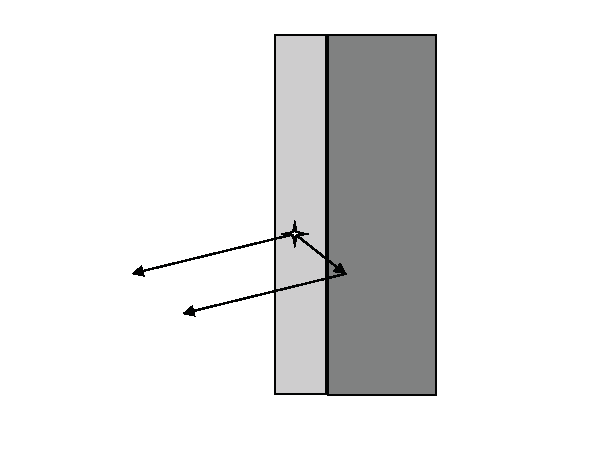
\includegraphics[scale=0.8]{DustyOpenGeometry}
\caption[Dusty open geometry]{
\label{fig:DustyOpenGeometry}The geometry assumed
in an open dusty geometry.
The lightly
shaded area is the H$^+$ region,
and is a layer on the surface of an infinitely
optically thick molecular cloud, the dark area on the right.
Light can
be emitted from the illuminated face of the cloud.
A fraction of the light
emitted towards the molecular cloud is reflected back towards the illuminated face. }
\end{figure}

\section{Continuum pumping contribution to line intensities}

Continuum pumping or fluorescence is included for all lines.
The contribution is only explicitly reported if the
\cdCommand{print line pump} command is entered.
Whether or not this contribution actually adds to the observed
line emission depends on the geometry.
Continuum pumping increases the
line emission if no related continuum absorption occurs.
This will be the
case if the continuum source is either not observed or not covered by
absorbing gas.
If absorbing gas covers an observed continuum source then
the situation is like the P Cygni problem, and pumping may not increase
the net intensity of the line at all (the absorption component will have
the same equivalent width as the associated emission).
The printed line
intensity includes this contribution unless the
\cdCommand{no induced processes} command is entered.
(The \cdCommand{no induced processes} command has many other effects and
so should only be used as a test.)

The output produced by the \cdCommand{save continuum} commands
does not include
the pumped part of the line contribution.
This is correct if the continuum
source is included in the beam, but is not if only the gas is observed.

\section{Column densities}

The column densities of all constituents are printed at the end of the
calculation.
Column densities within many excited states are also printed.
The excited states are identified with a `*'.
The table that
accompanies the description of the \cdTerm{cdColm} command
(see Table \ref{tab:cdColm_labels} on page
\pageref{tab:cdColm_labels} above)
identifies the various labels.

\section{A synthetic spectrum}

A table of emission-line intensities is part of the normal output.
Sometimes a synthetic spectrum, rather than a table, is desired.
Very coarse
spectra can be generated with the \cdCommand{save continuum} or
\cdCommand{save spectrum} commands,
but a detailed synthetic spectrum is not the main purpose of this output.

It is best to save the emission-line spectrum and then post-process this
data using your own software.  Then blends of lines can be synthesized at
any spectral resolution desired.
The spectrum can be save two ways.
The main block of emission-line intensities in the final printout
can be printed as a single column, which can be sorted by intensity
or wavelength (by using
options on the \cdCommand{print lines} command in Section 1 of this document).
The
\cdCommand{save spectrum} command includes a set of all lines with non-zero intensities.
Write a small program or script to read these tables and create a final
synthesized spectrum.

\section{Line profiles}

The observed line profile can be predicted by integrating the emissivity
of the line over the computed structure while taking the local velocity
structure into account.
The emissivity is obtained with the
\cdCommand{save lines emissivity} command,
described in Part 1 of this document.
This gives the
net emission, with units erg cm$^{-3}$~s$^{-1}$,
emitted by a unit volume of gas and
emergent from the cloud surface.
The total emission is the integral of
the emissivity.
An integral over radius will give the line intensity $4\pi J$
while an integral over volume will give the luminosity.

The observed profile will depend on the velocity field at each point
in the integration.
For static models this will be the Voigt function at
the local temperature and microturbulence.
For a dynamical model it will
include bulk motion of the gas.


